\documentclass[aspectratio=169]{beamer}
\usetheme{boxes}
\usepackage{bm}
\usepackage{booktabs}
\usepackage{amsfonts}
\usepackage{amssymb}
\usepackage{amsmath}
\usepackage{amsthm}
\usepackage{comment}
\usepackage{geometry}
% Removed algorithmic packages to avoid conflicts
\usepackage{graphicx}
\usepackage{subcaption}
\usepackage{tikz}
% \usepackage{physics} % Removed due to conflicts with essay-def
\usepackage{xcolor}
\usepackage{listings}
\usepackage{essay-def}
% Configure itemize for beamer
\setbeamertemplate{itemize item}{$\circ$}
\setbeamertemplate{itemize subitem}{\textbullet}
\usepackage[version=4]{mhchem}
\geometry{left=1cm,right=1cm}

% Define custom colors matching ByteDance style
\definecolor{highlight}{RGB}{220, 20, 60}
\definecolor{codegreen}{RGB}{0, 128, 0}
\definecolor{codepurple}{RGB}{128, 0, 128}

% Code listing style
\lstset{
  basicstyle=\ttfamily\footnotesize,
  keywordstyle=\color{blue},
  commentstyle=\color{codegreen},
  stringstyle=\color{codepurple},
  breaklines=true,
  frame=single,
  backgroundcolor=\color{gray!5}
}

\title[AI Agents]{AI Agents: From Tool Use to Autonomous Systems}
\subtitle{21 Days with Claude Code}
\author[J. Zhao \& CC]{Jiaxi Zhao (NUS) \& Claude Code (Anthropic)}
\date[\today]{\today}

\begin{document}

\begin{frame}
\titlepage
\end{frame}

\begin{frame}{Outline}
\tableofcontents
\end{frame}

% ==========================
% Section 1: What is Agent and Why Agent? (6 pages)
% ==========================
\section{What is Agent and Why Agent?}

\begin{frame}{What is an Agent?}
	\begin{block}{Formal Definition (Russell \& Norvig)}
		"An agent is anything that perceives its \textbf{environment} through sensors and acts upon that environment through \textbf{actuators}."
	\end{block}
	
	\vspace{0.3cm}
	
	\begin{columns}
		\column{0.5\textwidth}
		\textbf{Key Characteristics:}
		\begin{itemize}
			\item {\color{highlight}\textbf{Autonomy}}: Acts independently
			\item {\color{highlight}\textbf{Perception}}: Senses environment
			\item {\color{highlight}\textbf{Action}}: Changes environment
			\item {\color{highlight}\textbf{Goal-directed}}: Works toward objectives
		\end{itemize}
		
		\column{0.5\textwidth}
		\textbf{In AI Context:}
		\begin{itemize}
			\item Software that performs tasks autonomously
			\item Makes decisions to maximize goals
			\item Can learn and adapt over time
			\item Ranges from thermostats to LLMs
		\end{itemize}
	\end{columns}
	
	\vspace{0.3cm}
	
	\begin{center}
		\small
		{\color{gray}Etymology: From Latin \textit{agere} (to do) - "action on behalf of"}
	\end{center}
\end{frame}

\begin{frame}{Tool Use: Signal of Early Intelligence}
	\begin{columns}
		\column{\textwidth}
		\begin{itemize}
			\item {\color{highlight}\textbf{Anthropological perspective}}: Tool use marks cognitive revolution
			\begin{itemize}
				\item Stone tools $\rightarrow$ Agriculture $\rightarrow$ Writing systems
				\item Cognitive leap: from reactive to proactive behavior
			\end{itemize}
			\item {\color{highlight}\textbf{AI parallel}}: From language generation to action
			\begin{itemize}
				\item GPT-3 (2020): Pure text generation
				\item WebGPT (2021): Web browsing capability
				\item ChatGPT Plugins (2023): Tool ecosystem
				\item Claude Code (2024): Full IDE integration
			\end{itemize}
		\end{itemize}
	\end{columns}
\end{frame}

\begin{frame}{Eliminating Hallucination Through Grounding}
	\begin{itemize}
		\item {\color{highlight}\textbf{Problem}}: LLMs generate plausible but incorrect information
		\item {\color{highlight}\textbf{Solution}}: Ground responses in external tools and data
	\end{itemize}
	
	\begin{columns}
		\column{0.5\textwidth}
		\begin{block}{Without Tools}
			\small
			\texttt{Q: What is sqrt(144)?} \\
			\texttt{A: sqrt(144) = 13} \\
			{\color{red}$\times$ Hallucination}
		\end{block}
		
		\column{0.5\textwidth}
		\begin{block}{With Calculator Tool}
			\small
			\texttt{Thought: Use calculator} \\
			\texttt{Action: calc(sqrt(144))} \\
			\texttt{Result: 12} \\
			\texttt{A: sqrt(144) = 12} \\
			{\color{green}$\checkmark$ Grounded}
		\end{block}
	\end{columns}
	
	\vspace{0.5cm}
	% Presenter notes for the performance metrics
	\begin{itemize}
		\item WebGPT: 69\% preference vs Reddit answers
		% Note: "WebGPT uses web browsing to ground its answers with real sources.
		%        In human evaluation, 69% of users preferred WebGPT's referenced answers
		%        over crowd-sourced Reddit responses for factual questions."
		% TODO: move the following two items to their corresponding literature
		% review part, it does not fit well into this frame
		\item ReACT: Reduces error propagation in multi-hop QA  
		% Note: "ReACT interleaves reasoning with actions, preventing errors from
		%        compounding in complex multi-step questions. Each step is grounded
		%        in real tool outputs before proceeding to the next."
		\item Toolformer: Improved zero-shot performance across tasks
		% Note: "Toolformer teaches itself when to use tools without any examples.
		%        This self-supervised approach means it can handle new tasks immediately
		%        without needing task-specific training or demonstrations."
	\end{itemize}
	
	\begin{block}{Presenter Note}
		\footnotesize
		\textit{Key message: Each system shows how grounding LLMs with tools dramatically improves reliability. WebGPT proves users trust tool-backed answers, ReACT shows tools prevent cascading errors, and Toolformer demonstrates that models can learn tool use autonomously.}
	\end{block}
\end{frame}

\begin{frame}{Environmental Interaction Paradigm}
	\begin{center}
		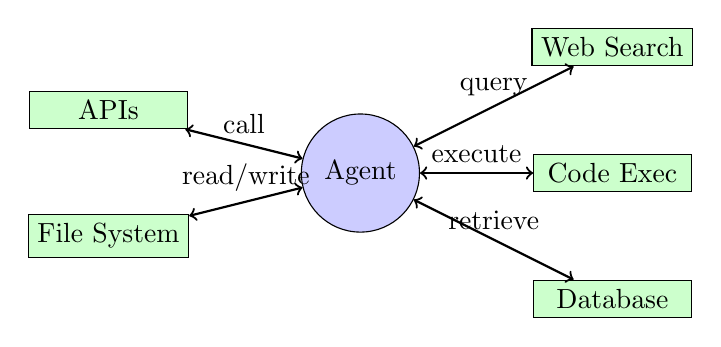
\begin{tikzpicture}[scale=0.8]
			% Agent
			\node[circle, draw, fill=blue!20, minimum size=1.5cm] (agent) at (0,0) {Agent};
			
			% Environment components
			\node[rectangle, draw, fill=green!20, minimum width=2cm] (web) at (4,2) {Web Search};
			\node[rectangle, draw, fill=green!20, minimum width=2cm] (code) at (4,0) {Code Exec};
			\node[rectangle, draw, fill=green!20, minimum width=2cm] (db) at (4,-2) {Database};
			\node[rectangle, draw, fill=green!20, minimum width=2cm] (api) at (-4,1) {APIs};
			\node[rectangle, draw, fill=green!20, minimum width=2cm] (file) at (-4,-1) {File System};
			
			% Arrows
			\draw[<->, thick] (agent) -- (web) node[midway, above] {query};
			\draw[<->, thick] (agent) -- (code) node[midway, above] {execute};
			\draw[<->, thick] (agent) -- (db) node[midway, above] {retrieve};
			\draw[<->, thick] (agent) -- (api) node[midway, above] {call};
			\draw[<->, thick] (agent) -- (file) node[midway, above] {read/write};
		\end{tikzpicture}
	\end{center}
	
	\begin{itemize}
		\item {\color{highlight}\textbf{Perception}}: Read from environment (search, query, read)
		\item {\color{highlight}\textbf{Action}}: Modify environment (write, execute, call)
		\item {\color{highlight}\textbf{Learning}}: Adapt based on feedback
	\end{itemize}
\end{frame}

\begin{frame}{RL Perspective: Agents as Policies}
	\begin{columns}
		\column{0.6\textwidth}
		\begin{itemize}
			\item {\color{highlight}\textbf{MDP Formulation}}:
			\begin{itemize}
				\item State $s$: Context + Environment state
				\item Action $a$: Tool calls, text generation
				\item Reward $r$: Task completion, human feedback
				\item Policy $\pi$: LLM with prompting strategy
			\end{itemize}
			\item {\color{highlight}\textbf{Training Methods}}:
			\begin{itemize}
				\item Imitation Learning (WebGPT)
				\item RLHF (Constitutional AI)
				\item Self-play (AutoGPT iterations)
			\end{itemize}
		\end{itemize}
		Are you sure this correspondence is precise, e.g. WebGPT uses imitation learning?
		
		\column{0.4\textwidth}
		\begin{block}{Agent Loop}
			\footnotesize
			\texttt{while not done:}\\
			\texttt{\ \ s = observe()}\\
			\texttt{\ \ a = $\pi$(s)}\\
			\texttt{\ \ s', r = env.step(a)}\\
			\texttt{\ \ update(s, a, r, s')}
		\end{block}
	\end{columns}
	
	\vspace{0.3cm}
	\begin{itemize}
		\item ReACT: 34\% improvement over RL baselines on ALFWorld
		\item Key insight: Language as both thought and action space
	\end{itemize}
\end{frame}

\begin{frame}{Evolution: From Prompting to Autonomy}
	\begin{center}
		\begin{tabular}{|l|c|c|c|c|}
			\hline
			\textbf{Capability} & \textbf{Prompting} & \textbf{Tool Use} & \textbf{Agents} & \textbf{Autonomous} \\
			\hline
			User Control & High & Medium & Low & Minimal \\
			Context Length & Limited & Limited & Extended & Unlimited* \\
			Error Recovery & Manual & Manual & Semi-auto & Automatic \\
			Task Complexity & Simple & Medium & Complex & Very Complex \\
			\hline
			\textbf{Example} & ChatGPT & Plugins & ReACT & AutoGPT \\
			\hline
		\end{tabular}
	\end{center}
	
	\vspace{0.5cm}
	
	\begin{itemize}
		\item {\color{highlight}\textbf{Prompting Era}} (2020-2022): Chain-of-thought, few-shot learning
		\item {\color{highlight}\textbf{Tool Use Era}} (2022-2023): Function calling, structured outputs
		\item {\color{highlight}\textbf{Agent Era}} (2023-2024): Planning, memory, reflection
		\item {\color{highlight}\textbf{Autonomous Era}} (2024-): Self-directed, continuous learning
	\end{itemize}
	
	\small
	*Via memory management systems like MemGPT
\end{frame}

% ==========================
% Section 2: How to Build Agent? (5 pages)
% ==========================
\section{How to Build Agent?}

\begin{frame}[fragile]{Tool Use Mechanism: From Text to Action}
	\begin{block}{Pattern Recognition for Tool Calls}
		LLMs output text $\rightarrow$ System recognizes patterns $\rightarrow$ Triggers tool execution
	\end{block}
	
	\begin{columns}
		\column{0.5\textwidth}
		\textbf{OpenAI Function Calling:}
		\begin{lstlisting}[basicstyle=\tiny]
{
  "role": "assistant",
  "content": null,
  "function_call": {
    "name": "get_weather",
    "arguments": "{\"location\": \"SF\"}"
  }
}
		\end{lstlisting}
		
		\column{0.5\textwidth}
		\textbf{ReACT Format:}
		\begin{lstlisting}[basicstyle=\tiny]
Thought: Need weather info
Action: weather_api
Action Input: San Francisco
Observation: 72F, sunny
Thought: I have the answer
		\end{lstlisting}
	\end{columns}
	
	\vspace{0.3cm}
	\begin{itemize}
		\item {\color{highlight}\textbf{JSON Schema}}: Structured output for reliable parsing
		\item {\color{highlight}\textbf{XML Tags}}: Claude's tool use format
		\item {\color{highlight}\textbf{Special Tokens}}: Toolformer's API call tokens
	\end{itemize}
\end{frame}

\begin{frame}[fragile]{MCP: Model Context Protocol}
	\begin{columns}
		\column{0.6\textwidth}
		\begin{itemize}
			\item {\color{highlight}\textbf{Standardized protocol}} for LLM-tool communication
			\item {\color{highlight}\textbf{Key Components}}:
			\begin{itemize}
				\item Resource discovery
				\item Tool registration
				\item Execution sandbox
				\item Result formatting
			\end{itemize}
			\item {\color{highlight}\textbf{Benefits}}:
			\begin{itemize}
				\item Tool interoperability
				\item Security isolation
				\item Consistent interfaces
			\end{itemize}
		\end{itemize}
		
		\column{0.4\textwidth}
		\begin{lstlisting}[language=python, basicstyle=\tiny]
# MCP Tool Definition
@mcp_tool
def search(query: str) -> str:
    """Search the web"""
    return web_api.search(query)

# Auto-registered with LLM
tools = discover_tools()
llm.register(tools)
		\end{lstlisting}
	\end{columns}
	
	\vspace{0.3cm}
	\begin{block}{MCP in Claude Code}
		Dynamically loads environment-specific tools at runtime, enabling IDE integration, file system access, and custom tool extensions
	\end{block}
\end{frame}

\begin{frame}{Agentic Workflows}
	\begin{center}
		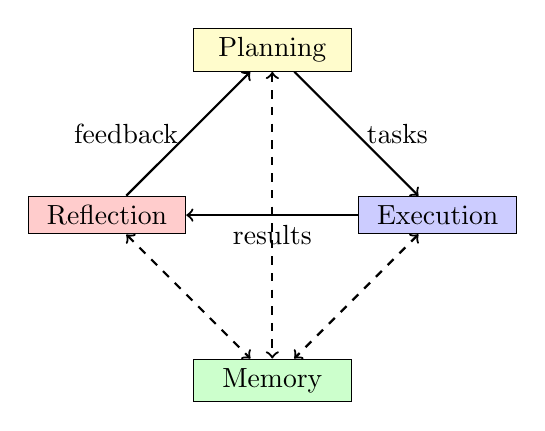
\begin{tikzpicture}[scale=0.7]
			% Planning
			\node[rectangle, draw, fill=yellow!20, minimum width=2cm] (plan) at (0,3) {Planning};
			
			% Execution
			\node[rectangle, draw, fill=blue!20, minimum width=2cm] (exec) at (3,0) {Execution};
			
			% Reflection
			\node[rectangle, draw, fill=red!20, minimum width=2cm] (reflect) at (-3,0) {Reflection};
			
			% Memory
			\node[rectangle, draw, fill=green!20, minimum width=2cm] (memory) at (0,-3) {Memory};
			
			% Arrows
			\draw[->, thick] (plan) -- (exec) node[midway, right] {tasks};
			\draw[->, thick] (exec) -- (reflect) node[midway, below] {results};
			\draw[->, thick] (reflect) -- (plan) node[midway, left] {feedback};
			
			\draw[<->, thick, dashed] (plan) -- (memory);
			\draw[<->, thick, dashed] (exec) -- (memory);
			\draw[<->, thick, dashed] (reflect) -- (memory);
		\end{tikzpicture}
	\end{center}
	
	\begin{columns}
		\column{0.5\textwidth}
		\begin{itemize}
			\item {\color{highlight}\textbf{Planning}}: Task decomposition
			\item {\color{highlight}\textbf{Execution}}: Tool calls, actions
		\end{itemize}
		
		\column{0.5\textwidth}
		\begin{itemize}
			\item {\color{highlight}\textbf{Reflection}}: Self-critique
			\item {\color{highlight}\textbf{Memory}}: Context persistence
		\end{itemize}
	\end{columns}
\end{frame}

\begin{frame}{Training Agents: Beyond Pre-training}
	\begin{tabular}{|l|p{3cm}|p{3cm}|p{3cm}|}
		\hline
		\textbf{Stage} & \textbf{Pre-training} & \textbf{Fine-tuning} & \textbf{Agent Training} \\
		\hline
		\textbf{Objective} & Next token prediction & Task-specific & Tool use + Planning \\
		\hline
		\textbf{Data} & Web text & Labeled examples & Trajectories \\
		\hline
		\textbf{Scale} & Trillions of tokens & Thousands & Millions of steps \\
		\hline
		\textbf{Method} & Self-supervised & Supervised & IL/RL/Self-play \\
		\hline
	\end{tabular}
	
	\vspace{0.5cm}
	
	\begin{itemize}
		\item {\color{highlight}\textbf{Imitation Learning}}: Learn from human demonstrations
		\begin{itemize}
			\item WebGPT: 6K demonstrations of web browsing
		\end{itemize}
		\item {\color{highlight}\textbf{Reinforcement Learning}}: Optimize for task rewards
		\begin{itemize}
			\item RLHF for preference alignment
		\end{itemize}
		\item {\color{highlight}\textbf{Self-improvement}}: Generate and learn from own data
		\begin{itemize}
			\item Toolformer: Self-supervised API call insertion
		\end{itemize}
	\end{itemize}
\end{frame}

\begin{frame}[fragile]{Agent Frameworks: LangChain \& LangGraph}
	\begin{columns}
		\column{0.5\textwidth}
		\textbf{LangChain:}
		\begin{itemize}
			\item {\color{highlight}Chain-based} architecture
			\item Sequential tool execution
			\item Pre-built components
		\end{itemize}
		\begin{lstlisting}[language=python, basicstyle=\tiny]
from langchain import LLMChain

chain = LLMChain(
    llm=ChatOpenAI(),
    tools=[search, calculator],
    memory=ConversationMemory()
)
result = chain.run(query)
		\end{lstlisting}
		
		\column{0.5\textwidth}
		\textbf{LangGraph:}
		\begin{itemize}
			\item {\color{highlight}Graph-based} workflows
			\item Conditional branching
			\item State machines
		\end{itemize}
		\begin{lstlisting}[language=python, basicstyle=\tiny]
from langgraph import StateGraph

graph = StateGraph()
graph.add_node("plan", planner)
graph.add_node("execute", executor)
graph.add_edge("plan", "execute")
graph.compile()
		\end{lstlisting}
	\end{columns}
	
	\vspace{0.3cm}
	\begin{block}{Framework Comparison}
		\small
		\begin{itemize}
			\item \textbf{AutoGPT}: Fully autonomous, self-prompting
			\item \textbf{BabyAGI}: Task queue management
			\item \textbf{CrewAI}: Multi-agent collaboration
		\end{itemize}
	\end{block}
\end{frame}

% ==========================
% Section 3: Agent Literature Review (5 pages)
% ==========================
\section{Agent Literature Review}

\begin{frame}{ReACT: Synergizing Reasoning and Acting}
	\begin{columns}
		\column{0.6\textwidth}
		\textbf{Key Innovation:} Interleaved reasoning traces and actions
		
		\begin{block}{ReACT Trace Example}
			\footnotesize
			\texttt{Question: What is the elevation of Mt. Everest?}\\
			\texttt{Thought: I need to search for Mt. Everest}\\
			\texttt{Action: search[Mt. Everest]}\\
			\texttt{Observation: Mt. Everest is Earth's highest mountain}\\
			\texttt{Thought: I need the specific elevation}\\
			\texttt{Action: lookup[elevation]}\\
			\texttt{Observation: 8,849 meters (29,032 ft)}\\
			\texttt{Thought: I have the answer}\\
			\texttt{Answer: 8,849 meters}
		\end{block}
		
		\column{0.4\textwidth}
		\textbf{Results:}
		\begin{itemize}
			\item HotpotQA: {\color{highlight}27\% improvement}
			\item ALFWorld: {\color{highlight}34\% over RL}
			\item WebShop: {\color{highlight}10\% improvement}
		\end{itemize}
		
		\textbf{Contributions:}
		\begin{itemize}
			\item Reasoning guides action
			\item Actions ground reasoning
			\item Human-interpretable
		\end{itemize}
	\end{columns}
	
	\vspace{0.2cm}
	\small
	Yao et al., ICLR 2023
\end{frame}

\begin{frame}[fragile]{MemGPT: Virtual Context Management}
	\begin{columns}
		\column{0.5\textwidth}
		\textbf{OS-Inspired Memory Hierarchy:}
		\begin{itemize}
			\item {\color{highlight}Main context}: Active working memory
			\item {\color{highlight}External storage}: Unlimited capacity
			\item {\color{highlight}Paging}: Move data between tiers
		\end{itemize}
		
		\begin{block}{Memory Operations}
			\footnotesize
			\begin{lstlisting}[basicstyle=\tiny]
# Page fault - need external data
if not in_context(info):
    page = load_from_storage(info)
    evict_lru_page()
    add_to_context(page)
			\end{lstlisting}
		\end{block}
		
		\column{0.5\textwidth}
		\begin{center}
			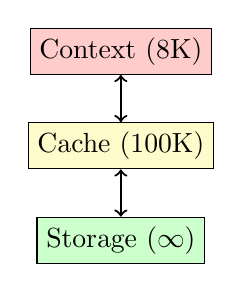
\begin{tikzpicture}[scale=0.6]
				\node[rectangle, draw, fill=red!20] (ctx) at (0,2) {Context (8K)};
				\node[rectangle, draw, fill=yellow!20] (cache) at (0,0) {Cache (100K)};
				\node[rectangle, draw, fill=green!20] (disk) at (0,-2) {Storage ($\infty$)};
				
				\draw[<->, thick] (ctx) -- (cache);
				\draw[<->, thick] (cache) -- (disk);
			\end{tikzpicture}
		\end{center}
		
		\textbf{Applications:}
		\begin{itemize}
			\item Document analysis beyond context
			\item Multi-session conversations
			\item Persistent agent memory
		\end{itemize}
	\end{columns}
	
	\vspace{0.3cm}
	\small
	Packer et al., October 2023
\end{frame}

\begin{frame}{Toolformer: Self-Supervised Tool Learning}
	\textbf{Core Innovation:} LLMs teach themselves when and how to use tools
	
	\begin{columns}
		\column{0.5\textwidth}
		\begin{block}{API Call Format}
			\footnotesize
			\texttt{The weather is <API>}\\
			\texttt{weather("New York")}\\
			\texttt{</API> 72°F today}
		\end{block}
		
		\textbf{Training Process:}
		\begin{itemize}
			\item[1.] Sample API calls positions
			\item[2.] Execute and evaluate utility
			\item[3.] Fine-tune on useful calls
		\end{itemize}
		
		\column{0.5\textwidth}
		\textbf{Tools Integrated:}
		\begin{itemize}
			\item Calculator
			\item QA System
			\item Search Engines
			\item Translation
			\item Calendar
		\end{itemize}
		
		\textbf{Results:}
		\begin{itemize}
			\item {\color{highlight}Zero-shot} improvements
			\item Maintains language ability
			\item Competitive with larger models
		\end{itemize}
	\end{columns}
	
	\vspace{0.3cm}
	\small
	Schick et al., Meta AI, February 2023
\end{frame}

\begin{frame}{WebGPT: Browser-Assisted QA}
	\begin{columns}
		\column{0.6\textwidth}
		\textbf{First large-scale web-browsing LLM}
		
		\begin{itemize}
			\item Text-based browser environment
			\item Imitation learning from humans
			\item Reference-backed answers
		\end{itemize}
		
		\begin{block}{Browser Actions}
			\small
			\begin{itemize}
				\item \texttt{search(query)}
				\item \texttt{click(link)}
				\item \texttt{quote(text)}
				\item \texttt{scroll()}
				\item \texttt{back()}
			\end{itemize}
		\end{block}
		
		\column{0.4\textwidth}
		\textbf{Training Data:}
		\begin{itemize}
			\item 6K demonstrations
			\item 20K comparisons
			\item Human feedback
		\end{itemize}
		
		\textbf{Performance:}
		\begin{itemize}
			\item {\color{highlight}56\%} preferred over humans
			\item {\color{highlight}69\%} vs Reddit answers
			\item Factual with citations
		\end{itemize}
	\end{columns}
	
	\vspace{0.3cm}
	\small
	Nakano et al., OpenAI, December 2021
\end{frame}

\begin{frame}{Comparative Analysis}
	\begin{center}
		\small
		\begin{tabular}{|l|c|c|c|c|}
			\hline
			\textbf{Method} & \textbf{Memory} & \textbf{Tools} & \textbf{Training} & \textbf{Key Innovation} \\
			\hline
			ReACT & Limited & External & Few-shot & Reasoning traces \\
			MemGPT & {\color{highlight}Unlimited} & Basic & N/A & Virtual memory \\
			Toolformer & Limited & {\color{highlight}5 types} & Self-supervised & Auto tool learning \\
			WebGPT & Limited & Browser & {\color{highlight}RLHF} & Web grounding \\
			AutoGPT & Short+Long & Extensible & None & {\color{highlight}Self-prompting} \\
			\hline
		\end{tabular}
	\end{center}
	
	\vspace{0.5cm}
	
	\textbf{Current Trends:}
	\begin{columns}
		\column{0.5\textwidth}
		\begin{itemize}
			\item Multi-agent systems
			\item Continuous learning
			\item Tool creation
		\end{itemize}
		
		\column{0.5\textwidth}
		\begin{itemize}
			\item Code generation agents
			\item Embodied agents
			\item Scientific discovery
		\end{itemize}
	\end{columns}
	
	\vspace{0.3cm}
	\textbf{Open Challenges:} Reliability, safety, evaluation metrics, cost
\end{frame}

% ==========================
% Section 4: Case Study - Claude Code (15 pages)
% ==========================
\section{Case Study: Claude Code}

\begin{frame}[fragile]{Claude Code: Introduction}
	\begin{columns}
		\column{0.6\textwidth}
		\textbf{What is Claude Code?}
		\begin{itemize}
			\item {\color{highlight}Anthropic's official CLI} for Claude
			\item Full IDE integration
			\item Autonomous coding agent
			\item Released 2024
		\end{itemize}
		
		\textbf{Key Capabilities:}
		\begin{itemize}
			\item Read/write files
			\item Execute commands
			\item Search codebases
			\item Run tests
			\item Git operations
			\item Web browsing
		\end{itemize}
		
		\column{0.4\textwidth}
		\begin{block}{Installation}
			\footnotesize
			\begin{lstlisting}[language=bash]
# Install Claude Code
npm install -g @anthropic/claude-code

# Initialize
claude-code init

# Start coding
claude-code "fix the bug in main.py"
			\end{lstlisting}
		\end{block}
		
		\textbf{Models Used:}
		\begin{itemize}
			\item Haiku 3.5 (quota check)
			\item Sonnet 4 (main agent)
			\item Opus 4.1 (complex tasks)
		\end{itemize}
	\end{columns}
\end{frame}

\begin{frame}{Architecture: Multi-Agent System}
	\begin{center}
		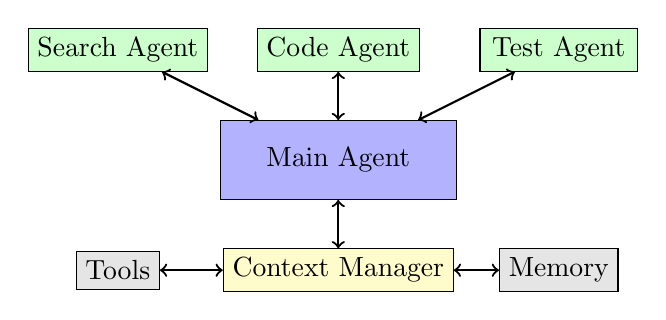
\begin{tikzpicture}[scale=0.7]
			% Main Agent
			\node[rectangle, draw, fill=blue!30, minimum width=3cm, minimum height=1cm] (main) at (0,0) {Main Agent};
			
			% Sub-agents
			\node[rectangle, draw, fill=green!20, minimum width=2cm] (search) at (-4,2) {Search Agent};
			\node[rectangle, draw, fill=green!20, minimum width=2cm] (code) at (0,2) {Code Agent};
			\node[rectangle, draw, fill=green!20, minimum width=2cm] (test) at (4,2) {Test Agent};
			
			% Context Manager
			\node[rectangle, draw, fill=yellow!20, minimum width=2cm] (context) at (0,-2) {Context Manager};
			
			% Tools
			\node[rectangle, draw, fill=gray!20] (tools) at (-4,-2) {Tools};
			\node[rectangle, draw, fill=gray!20] (memory) at (4,-2) {Memory};
			
			% Connections
			\draw[<->, thick] (main) -- (search);
			\draw[<->, thick] (main) -- (code);
			\draw[<->, thick] (main) -- (test);
			\draw[<->, thick] (main) -- (context);
			\draw[<->, thick] (context) -- (tools);
			\draw[<->, thick] (context) -- (memory);
		\end{tikzpicture}
	\end{center}
	
	\begin{itemize}
		\item {\color{highlight}\textbf{Main Agent}}: Orchestrates overall task
		\item {\color{highlight}\textbf{Sub-agents}}: Handle specific subtasks in isolation
		\item {\color{highlight}\textbf{Context Manager}}: Optimizes token usage
	\end{itemize}
\end{frame}

\begin{frame}{Reverse Engineering: System Prompts}
	\textbf{Key System Prompt Elements:}
	
	\begin{block}{Core Instructions}
		\footnotesize
		\begin{itemize}
			\item "You are Claude Code, Anthropic's official CLI for Claude"
			\item "Be concise, direct, and to the point"
			\item "Minimize output tokens while maintaining quality"
			\item "Use tools to complete tasks, not for communication"
		\end{itemize}
	\end{block}
	
	\textbf{Behavioral Guidelines:}
	\begin{columns}
		\column{0.5\textwidth}
		\begin{itemize}
			\item {\color{highlight}Proactive}: Use TODO lists
			\item {\color{highlight}Defensive}: Follow conventions
			\item {\color{highlight}Efficient}: Batch operations
		\end{itemize}
		
		\column{0.5\textwidth}
		\begin{itemize}
			\item {\color{highlight}Safe}: Never commit without asking
			\item {\color{highlight}Clear}: Explain complex commands
			\item {\color{highlight}Adaptive}: Learn from context
		\end{itemize}
	\end{columns}
	
	\small
	Source: github.com/Yuyz0112/claude-code-reverse
\end{frame}

\begin{frame}{Agentic Workflow}
	\begin{itemize}
		\item[1.] {\color{highlight}\textbf{Quota Check}} (Haiku 3.5)
		\begin{itemize}
			\item Lightweight API verification
			\item Context initialization
		\end{itemize}
		
		\item[2.] {\color{highlight}\textbf{Task Analysis}} (Main Agent)
		\begin{itemize}
			\item Parse user request
			\item Create TODO list
			\item Plan execution strategy
		\end{itemize}
		
		\item[3.] {\color{highlight}\textbf{Execution Loop}}
		\begin{itemize}
			\item Execute tools in parallel when possible
			\item Update TODO status
			\item Handle errors and retry
		\end{itemize}
		
		\item[4.] {\color{highlight}\textbf{Context Compaction}}
		\begin{itemize}
			\item Isolate "dirty context" in sub-agents
			\item Return only essential results
			\item Maintain conversation history
		\end{itemize}
	\end{itemize}
\end{frame}

\begin{frame}{TODO List: Dynamic Task Management}
	\begin{columns}
		\column{0.5\textwidth}
		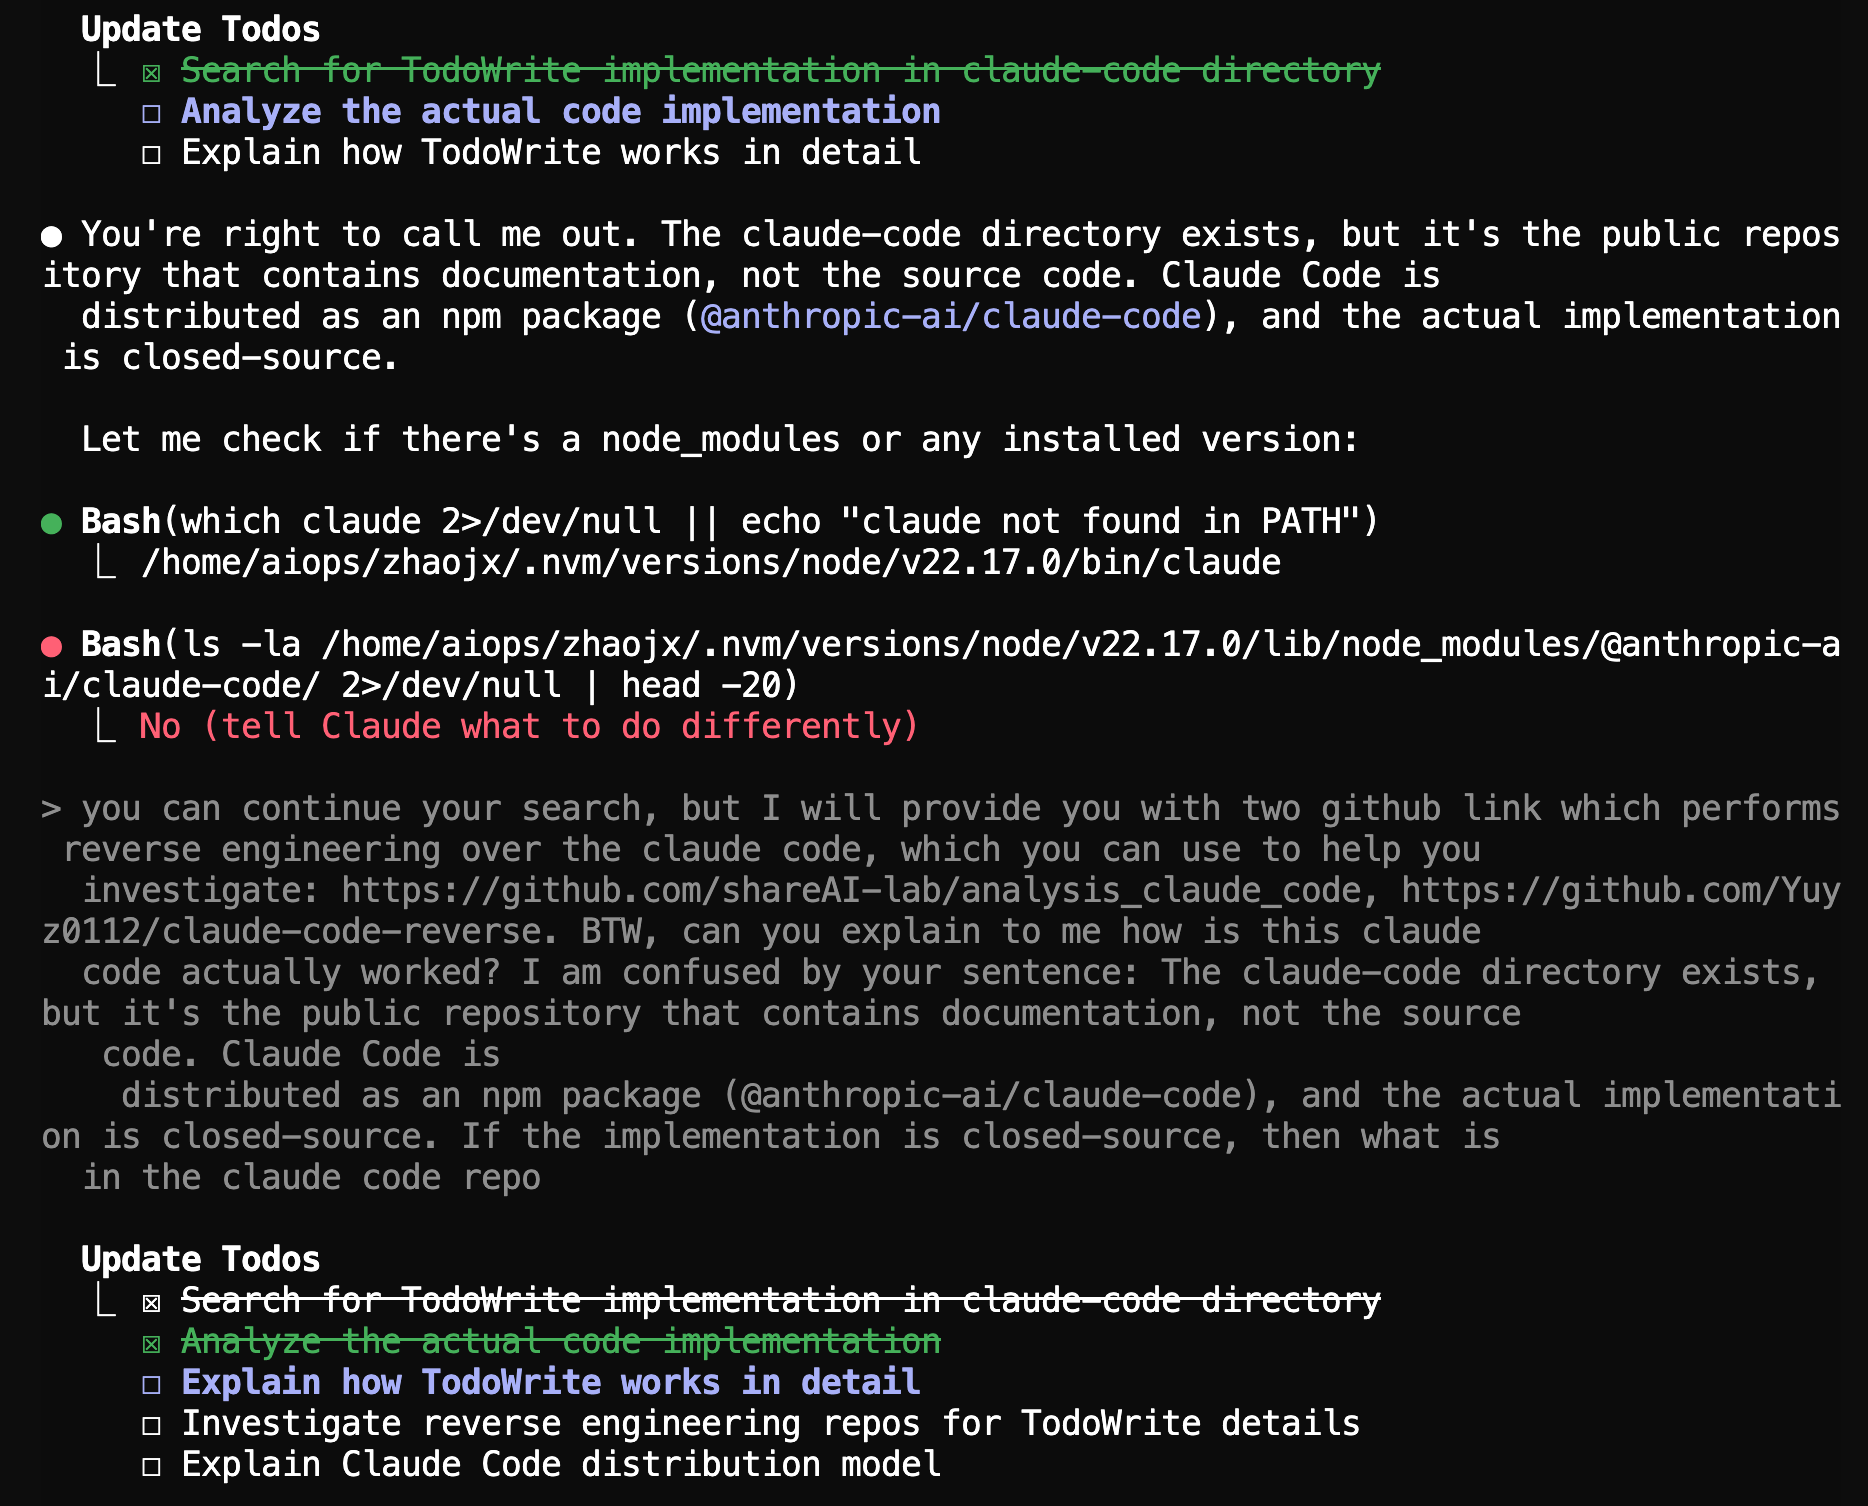
\includegraphics[width=\textwidth]{fig/TODO1.jpg}
		
		\column{0.5\textwidth}
		\textbf{Implementation:}
		\begin{itemize}
			\item Stored in \texttt{\~{}/.claude/todos/}
			\item JSON format
			\item Three states:
			\begin{itemize}
				\item \texttt{pending}
				\item \texttt{in\_progress}
				\item \texttt{completed}
			\end{itemize}
		\end{itemize}
		
		\textbf{Benefits:}
		\begin{itemize}
			\item User visibility
			\item Progress tracking
			\item Task decomposition
			\item Error recovery
		\end{itemize}
	\end{columns}
\end{frame}

\begin{frame}{TODO List: Real Example}
	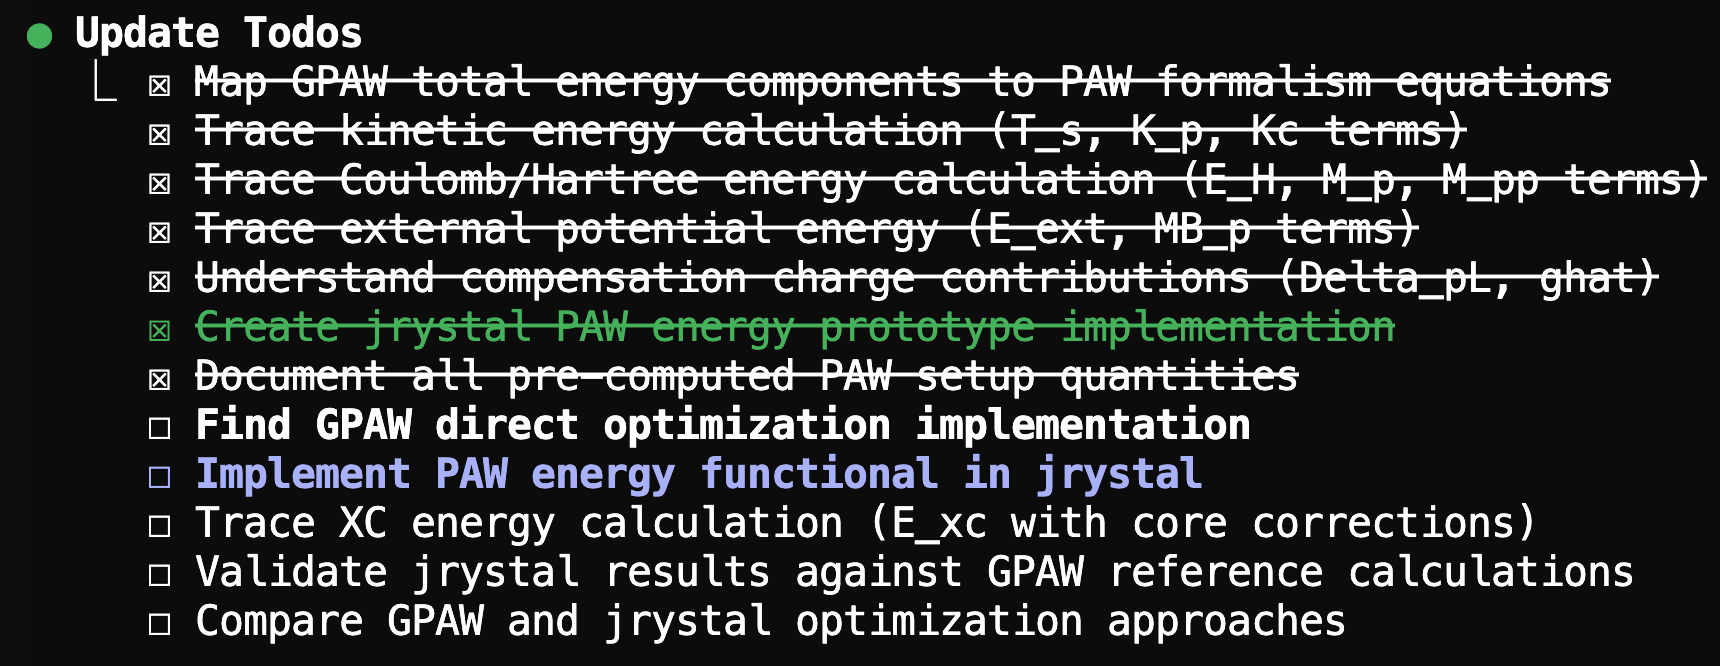
\includegraphics[width=0.8\textwidth]{fig/TODO2.jpg}
	
	\begin{itemize}
		\item {\color{highlight}Automatic creation} when task complexity detected
		\item {\color{highlight}Real-time updates} as work progresses
		\item {\color{highlight}Hierarchical} task breakdown
	\end{itemize}
\end{frame}

\begin{frame}[fragile]{Test Case: Scientific Computing (99\%)}
	\textbf{Task:} Read and understand complex numerical solver
	
	\begin{block}{Claude Code Performance}
		\begin{itemize}
			\item $\checkmark$ Identified algorithm structure
			\item $\checkmark$ Explained mathematical foundations
			\item $\checkmark$ Found optimization opportunities
			\item $\checkmark$ Generated comprehensive documentation
		\end{itemize}
	\end{block}
	
	\begin{lstlisting}[language=python, basicstyle=\tiny]
# Claude correctly identified spectral method
def spectral_solver(u, dt, nu):
    """Solve 2D Navier-Stokes using FFT"""
    u_hat = fft2(u)
    # Claude: "Using semi-implicit time stepping 
    # for stability with explicit nonlinear terms"
    nonlinear = compute_nonlinear(u)
    u_hat = (u_hat + dt * fft2(nonlinear)) / (1 + nu * dt * k2)
    return ifft2(u_hat)
	\end{lstlisting}
\end{frame}

\begin{frame}[fragile]{Test Case: Environment Setup (99\%)}
	\textbf{Task:} Modify Docker configuration for ML pipeline
	
	\begin{columns}
		\column{0.5\textwidth}
		\begin{block}{Original Dockerfile}
			\footnotesize
			\begin{lstlisting}[basicstyle=\tiny]
FROM python:3.8
RUN pip install numpy
CMD ["python", "app.py"]
			\end{lstlisting}
		\end{block}
		
		\column{0.5\textwidth}
		\begin{block}{Claude's Modification}
			\footnotesize
			\begin{lstlisting}[basicstyle=\tiny]
FROM python:3.8-slim
WORKDIR /app
COPY requirements.txt .
RUN pip install --no-cache-dir -r requirements.txt
COPY . .
CMD ["python", "-u", "app.py"]
			\end{lstlisting}
		\end{block}
	\end{columns}
	
	\textbf{Improvements Made:}
	\begin{itemize}
		\item Used slim image (reduced size)
		\item Added proper layer caching
		\item Implemented best practices
		\item Added unbuffered output
	\end{itemize}
\end{frame}

\begin{frame}[fragile]{Test Case: Unit Testing}
	\textbf{Task:} Write comprehensive unit tests
	
	\begin{lstlisting}[language=python, basicstyle=\tiny]
# Claude generated test with edge cases
def test_matrix_operations():
    """Test matrix multiplication with various inputs"""
    # Test normal case
    assert multiply([[1,2],[3,4]], [[5,6],[7,8]]) == [[19,22],[43,50]]
    
    # Test identity
    I = [[1,0],[0,1]]
    A = [[1,2],[3,4]]
    assert multiply(A, I) == A
    
    # Test zero matrix
    Z = [[0,0],[0,0]]
    assert multiply(A, Z) == Z
    
    # Test dimension mismatch
    with pytest.raises(ValueError):
        multiply([[1,2]], [[1],[2],[3]])
	\end{lstlisting}
	
	{\color{highlight}Key: Clear interface + complete instructions = High success}
\end{frame}

\begin{frame}{Test Case: Debug NS Solver (40\%)}
	\textbf{Task:} Debug hand-written spectral solver for 2D Navier-Stokes
	
	\textbf{Challenges Encountered:}
	\begin{itemize}
		\item {\color{red}$\times$} Complex aliasing errors
		\item {\color{red}$\times$} Numerical stability issues  
		\item {\color{orange}$\triangle$} Identified problem areas
		\item {\color{red}$\times$} Could not fix without domain expertise
	\end{itemize}
	
	\textbf{Lesson:} Claude Code struggles with:
	\begin{itemize}
		\item Deep domain-specific knowledge
		\item Numerical analysis subtleties
		\item Complex debugging requiring intuition
	\end{itemize}
\end{frame}

\begin{frame}{Test Case: Hydra Configuration (20\%)}
	\textbf{Task:} Set up Hydra for multi-run experiments
	
	\textbf{Issues:}
	\begin{itemize}
		\item {\color{red}$\times$} Misunderstood Hydra's configuration structure
		\item {\color{red}$\times$} Generated incorrect sweep syntax
		\item {\color{red}$\times$} Failed to handle composition properly
	\end{itemize}
	
	\textbf{Root Cause:}
	\begin{itemize}
		\item Limited training data on Hydra
		\item Complex configuration inheritance
		\item Framework-specific patterns
	\end{itemize}
\end{frame}

\begin{frame}{Claude Code as a Tool for Humans}
	\textbf{Key Insight:} {\color{highlight}Dramatically lowers barriers} for many tasks
	
	\begin{columns}
		\column{0.5\textwidth}
		\textbf{Before Claude Code:}
		\begin{itemize}
			\item Hours reading documentation
			\item Manual environment setup
			\item Trial-and-error debugging
			\item Context switching overhead
		\end{itemize}
		
		\column{0.5\textwidth}
		\textbf{With Claude Code:}
		\begin{itemize}
			\item Instant codebase understanding
			\item Automated setup scripts
			\item Guided exploration
			\item Maintained context
		\end{itemize}
	\end{columns}
	
	\vspace{0.5cm}
	
	\begin{block}{Best Use Cases}
		\begin{itemize}
			\item {\color{highlight}Learning new repositories}: Navigate unfamiliar codebases
			\item {\color{highlight}Environment setup}: Docker, dependencies, configuration
			\item {\color{highlight}Boilerplate generation}: Tests, documentation, CI/CD
			\item {\color{highlight}Refactoring}: Systematic code improvements
		\end{itemize}
	\end{block}
\end{frame}

\begin{frame}{Lessons from Claude Code}
	\textbf{Architectural Insights:}
	\begin{itemize}
		\item {\color{highlight}Multi-agent} design scales better than monolithic
		\item {\color{highlight}Context management} is crucial for long tasks
		\item {\color{highlight}TODO lists} provide structure and visibility
	\end{itemize}
	
	\textbf{Practical Implications:}
	\begin{itemize}
		\item Works best with {\color{highlight}clear specifications}
		\item Excels at {\color{highlight}well-defined tasks}
		\item Struggles with {\color{highlight}domain-specific expertise}
	\end{itemize}
	
	\textbf{Future Directions:}
	\begin{itemize}
		\item Better memory systems (MemGPT-style)
		\item Improved error recovery
		\item Domain-specific fine-tuning
		\item Multi-modal capabilities (diagrams, UI)
	\end{itemize}
\end{frame}

\begin{frame}{Performance Summary}
	\begin{center}
		\begin{tabular}{|l|c|p{5cm}|}
			\hline
			\textbf{Task Type} & \textbf{Score} & \textbf{Key Factors} \\
			\hline
			Code Reading & {\color{green}99\%} & Pattern recognition, documentation \\
			Environment Setup & {\color{green}99\%} & Standard practices, clear goals \\
			Unit Testing & {\color{green}95\%} & Clear interfaces, specifications \\
			Complex Debug & {\color{orange}40\%} & Needs domain expertise \\
			Framework Config & {\color{red}20\%} & Limited training data \\
			Novel Algorithms & {\color{red}N/A} & Beyond current capabilities \\
			\hline
		\end{tabular}
	\end{center}
	
	\vspace{0.5cm}
	
	\textbf{Key Takeaway:}
	\begin{center}
		\large
		{\color{highlight}Claude Code is a powerful amplifier for human developers,}\\
		{\color{highlight}not a replacement for domain expertise}
	\end{center}
\end{frame}


\begin{frame}{}
	\begin{center}
		\Huge Thank You!
		
		\vspace{1cm}
		
		\Large Questions?
	\end{center}
\end{frame}

\end{document}